The radiation damage created by \ac{HL-LHC} will become a big challenge for the innermost tracking detectors. After a large irradiation, all detector material will become trap limited with a \ac{MFP} below \SI{75}{\micro\meter}. The concept of a so called 3D-Detector is a possible way to highly increase the longevity of these materials. Its basic principle is shown in figure \vref{3d1}: In a planer detector the readout and bias electrodes are brought onto the front and back side of the sensor with a thickness $\Updelta$. The resulting drift distance L of the charge carriers is of the order of $\Updelta$. In the 3D detector the electrodes are put inside of the detector material so that the \acp{MIP} can travel the same distance $\Updelta$ in the material and therefore create the same amount charge carriers but L is heavily reduced. In case of diamond these electrode columns are drilled with a \SI{800}{\nano\meter} femtosecond laser which converts the diamond into a resistive mixture of carbon phases.\\

\begin{figure} 
	\centering
	\subfig[.43]{PlanarConcept.png}{.2}{planar}
	\begin{subfigure}{0.1\textwidth}  
		\centering 
		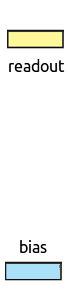
\includegraphics[height=.2\textheight]{LegendConcept.png}
		\vspace*{19pt}
	\end{subfigure}
	\subfig[.43]{3DConcept.png}{.2}{3D}
	\caption{Comparison of the planar and the 3D detector concepts}
	\label{3d1}
\end{figure}

\noindent In 2015 one of the first detectors was built out of a \ac{pCVD} diamond sensor which had a 3D detector as well as a strip detector on the same sensor. At this time the column efficiency was about \SI{92}{\%} and the 3D cells had a size of \SI{150x150}{\micro\meter}. This detector was already a success by showing a working 3D diamond detector. Its square cells are clearly visible and the measured signal for the thickness of \SI{500}{\micro\meter} was \SI{13500}{e} which is much higher than \SI{6900}{e} in the strip detector. The strip signal equates to a \ac{CCD} of \SI{192}{\micro\meter}. The measured charge in the 3D would have a \ac{CCD} in a planar detector of \SIrange{350}{375}{\micro\meter} which effectively means that more than \SI{75}{\%} of the created charge was collected for the first time in a \ac{pCVD} diamond. The according pulse height distributions are shown in \vref{3d2}.